\documentclass[compress]{beamer}
\usepackage{ifthen,verbatim}

\newcommand{\isnote}{}
\xdefinecolor{lightyellow}{rgb}{1.,1.,0.25}
\xdefinecolor{darkblue}{rgb}{0.1,0.1,0.7}

%% Uncomment this to get annotations
%% \def\notes{\addtocounter{page}{-1}
%%            \renewcommand{\isnote}{*}
%% 	   \beamertemplateshadingbackground{lightyellow}{white}
%%            \begin{frame}
%%            \frametitle{Notes for the previous page (page \insertpagenumber)}
%%            \itemize}
%% \def\endnotes{\enditemize
%% 	      \end{frame}
%%               \beamertemplateshadingbackground{white}{white}
%%               \renewcommand{\isnote}{}}

%% Uncomment this to not get annotations
\def\notes{\comment}
\def\endnotes{\endcomment}

\setbeamertemplate{navigation symbols}{}
\setbeamertemplate{headline}{\mbox{ } \hfill
\begin{minipage}{5.5 cm}
\vspace{-0.75 cm} \small
\end{minipage} \hfill
\begin{minipage}{4.5 cm}
\vspace{-0.75 cm} \small
\begin{flushright}
{Jim Pivarski \hspace{0.2 cm} \insertpagenumber\isnote/\pageref{numpages}}
\end{flushright}
\end{minipage}\mbox{\hspace{0.2 cm}}\includegraphics[height=1 cm]{../cmslogo} \hspace{0.1 cm} \includegraphics[height=1 cm]{../tamulogo} \hspace{0.01 cm} \vspace{-1.05 cm}}

\begin{document}
%% \begin{notes}
%% \item This is the annotated version of my talk.
%% \item If you want the version that I am presenting, download the one
%% labeled ``slides'' on Indico (or just ignore these yellow pages).
%% \item The annotated version is provided for extra detail and a written
%% record of comments that I intend to make orally.
%% \item Yellow notes refer to the content on the {\it previous} page.
%% \item All other slides are identical for the two versions.
%% \end{notes}

\small

%% \begin{frame}
%% \frametitle{Outline}
%% \begin{itemize}\setlength{\itemsep}{0.75 cm}
%% \item 
%% \end{itemize}
%% %% \hspace{-0.83 cm} \textcolor{darkblue}{\Large Outline2}
%% \end{frame}

\begin{frame}
\frametitle{General things}
\begin{itemize}
\item Our $h \to aa \to 4\mu$ paper has been accepted to PRD (without revisions)!

\item I've booked a flight to Houston: arrive Mon, Apr~5 (12:50~PM), depart Sat, Apr~10 (6:25~PM)
\begin{itemize}
\item still need rental car and hotel
\end{itemize}

\item List of current alignment projects:
\begin{itemize}\setlength{\itemsep}{0.1 cm}
\item \textcolor{darkblue}{Aysen:} optimize collisions alignment $|\vec{p}|$ cut.  If $p_T <
  10$~GeV muons are useful, we'll need to revise MuAlCalIsolatedMu
  data stream, which requires a new CMSSW release--- must be done well
  in advance of first 7~TeV reprocessing!
\item \textcolor{darkblue}{Aysen:} align DT chambers and CSC rings with 2010 cosmics
\item \textcolor{darkblue}{Vadim:} making alignment monitor public (e.g.\ for hardware alignment)
\item \textcolor{darkblue}{Vadim:} separate CSC ring alignment script
\item \textcolor{darkblue}{Jim:} help everyone with everything
\item \textcolor{darkblue}{Jim:} CSC-Overlaps alignment procedure re-write (next pages)
\end{itemize}

\end{itemize}
\end{frame}

\begin{frame}
\frametitle{CSC-Overlaps status}
\begin{itemize}
\item Mathematical generalization has been fully tested in a sandbox
  (little Python scripts to make sure that I know what I'm doing)
\begin{itemize}
\item details on next pages
\item cross-checked linear algebra solution with Minuit
\end{itemize}

\item Implemented and tested the above in CMSSW
\begin{itemize}
\item fully configurable by \_cfg
\item yields same results as scripts
\end{itemize}

\item Building the rest of the package around that
\begin{itemize}
\item CSC-Overlaps procedure is (and has always been) more complicated than Reference-Target
\item this is a procedure that really needs abstraction; classes to
  perform neighboring-chamber track fits, matrix-based alignment
  solution, separation of the calculation from the monitoring
  plots\ldots
\item not much to show right now because I'm programming
\end{itemize}

\item There will be a detailed Note describing both the mathematical
  formalism and the C++ implementation
\end{itemize}
\end{frame}

\begin{frame}
\frametitle{Mathematical formalism}

\vspace{0.3 cm}
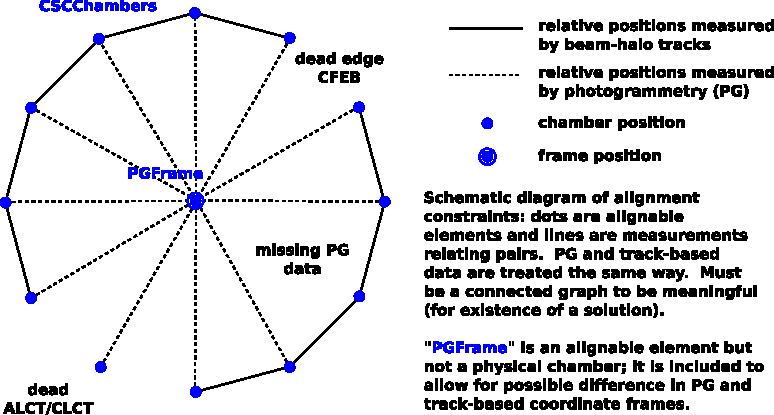
\includegraphics[width=\linewidth]{beamhalo-PG.pdf}

\scriptsize
\begin{itemize}
\item Solution is a minimization of $\displaystyle \chi^2 =
\sum_{\mbox{\scriptsize constraints}} \frac{(m_{ij} - A_i +
  A_j)^2}{{\sigma_{ij}}^2} + f(\lambda, A)$ \\ \vspace{0.1 cm} with respect to alignment
corrections $A$ (blue dots, above) where $m_{ij}$ and $\sigma_{ij}$ are
measurements with uncertainties (lines).

\item $f(\lambda, A)$ is a Lagrange multiplier to fix the overall reference frame.
\end{itemize}
\end{frame}

%% \section*{First section}
%% \begin{frame}
%% \begin{center}
%% \Huge \textcolor{blue}{First section}
%% \end{center}
%% \end{frame}

\begin{frame}
\frametitle{Mathematical formalism}

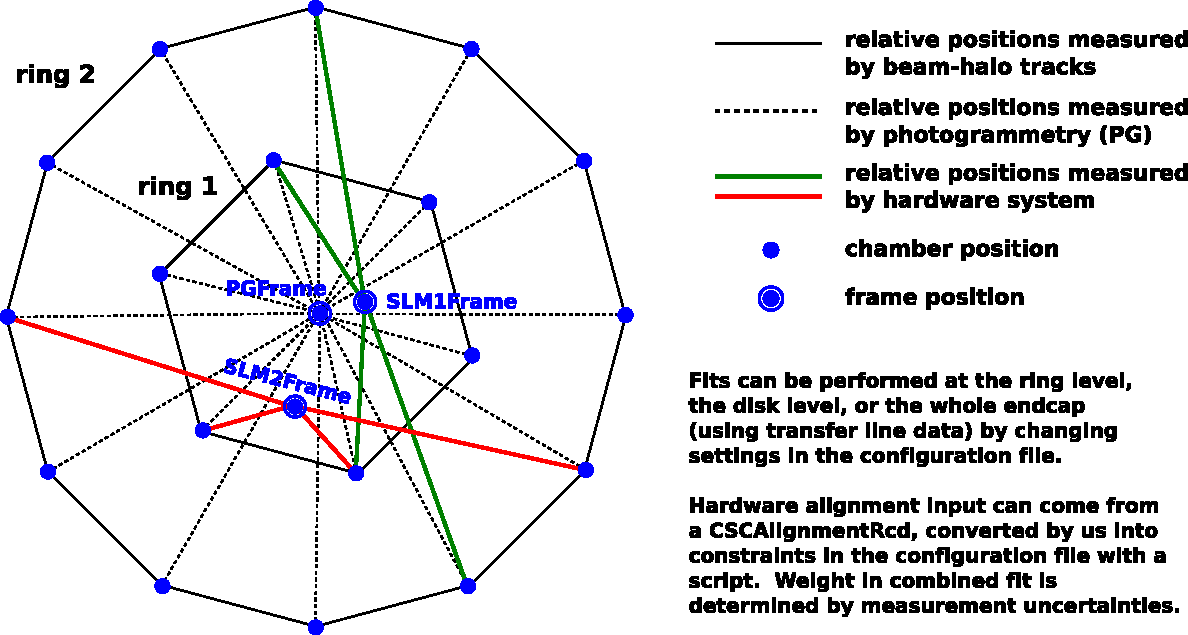
\includegraphics[width=\linewidth]{beamhalo-PG-SLM.pdf}

\scriptsize
\begin{itemize}
\item Formalism is general enough to include any statistically
  independent two-chamber constraints, in any configuration--- options for the future.

\item CSCRing-to-tracker alignment should also include a
  CSCDisk-to-tracker mode to preserve relative positions of ring 1 and
  2.  Vadim and I have talked about this--- it shouldn't be difficult.
\end{itemize}
\label{numpages}
\end{frame}

\end{document}
